\begin{center}
  \Large
  \textbf{BIOGRAFI PENULIS}
\end{center}

\addcontentsline{toc}{chapter}{BIOGRAFI PENULIS}

\vspace{2ex}

\begin{wrapfigure}{L}{0.3\textwidth}
  \centering
  \vspace{-3ex}
  % Ubah file gambar berikut dengan file foto dari mahasiswa
  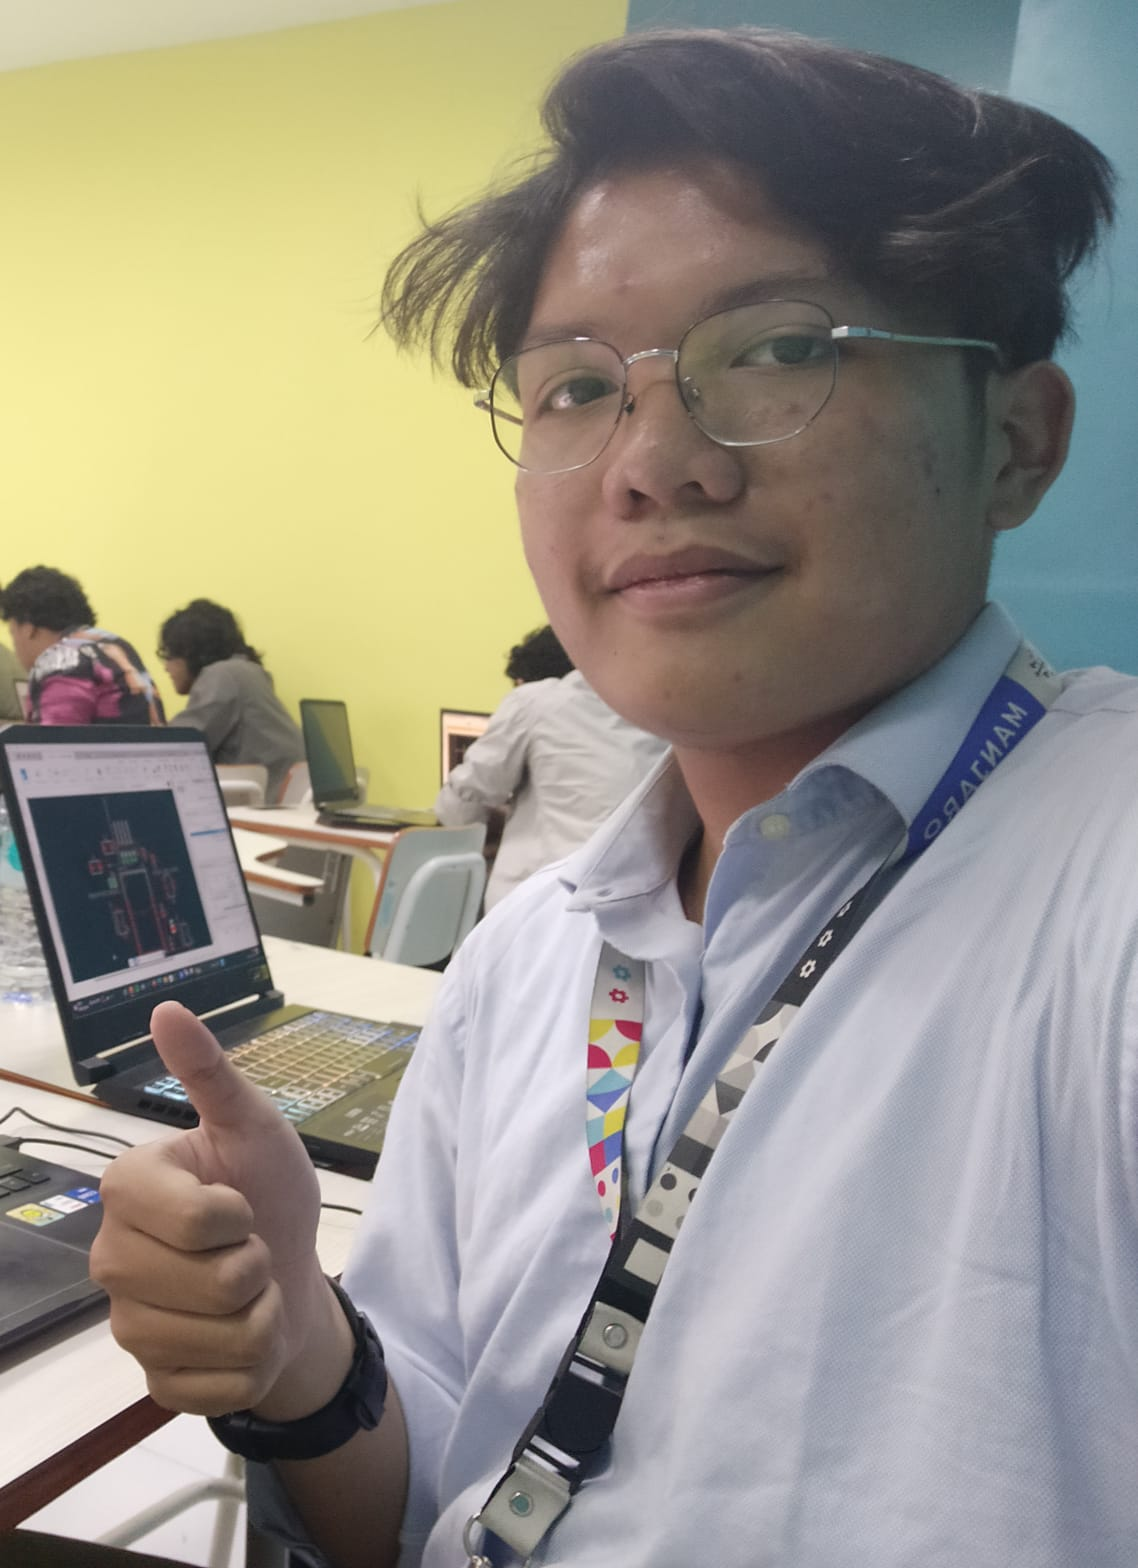
\includegraphics[width=0.3\textwidth]{BiografiPenulis/foto-formal.png}
  \vspace{-4ex}
\end{wrapfigure}

% Ubah kalimat berikut dengan biografi dari mahasiswa
\name{}, atau yang biasa dikenal sebagai Imanuel Daulat, merupakan mahasiswa Program Studi Teknik Komputer, Departemen Teknik Komputer, Fakultas Teknologi Elektro dan Informatika Cerdas, Institut Teknologi Sepuluh Nopember (ITS) angkatan 2022. Saat ini penulis menempuh perkuliahan pada semester akhir dan memiliki ketertarikan pada bidang analisis data, kecerdasan buatan, serta \textit{Machine Learning Operations} (MLOps).

Selama masa studi, penulis aktif mengembangkan kompetensi teknis yang berkaitan dengan pengolahan data, pengembangan model berbasis \textit{machine learning}, dan penerapan sistem berbasis data untuk mendukung proses pengambilan keputusan. Ketertarikan tersebut semakin berkembang melalui pengalaman profesional penulis di industri saat menjalani peran sebagai IT Operations \& Data Analyst Intern di Bank Mandiri Taspen, Jakarta. Dalam pengalaman tersebut, penulis berfokus pada optimalisasi query SQL Server serta pengembangan dashboard analitik menggunakan Tableau untuk mendukung kebutuhan analisis pada divisi internal perusahaan.

Pada penelitian tugas akhir ini, penulis mengangkat topik perancangan dan implementasi pipeline \textit{Machine Learning Operations} (MLOps) untuk operasionalisasi model prediktif risiko kredit. Topik ini dipilih karena sejalan dengan minat penulis pada bidang analisis data, kecerdasan buatan, dan penerapan sistem data di industri keuangan. Melalui penelitian ini, penulis berharap hasil yang dikembangkan dapat memberikan kontribusi awal terhadap penerapan sistem \textit{credit risk scoring} yang lebih terstruktur, transparan, dan adaptif terhadap perubahan data.
